\documentclass[tikz]{standalone}

\usepackage{tikz}
\usetikzlibrary{automata}

\begin{document}

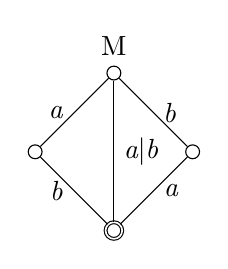
\begin{tikzpicture}
    \tikzstyle{every state}=[
        draw,
        shape=circle,
        inner sep=1pt,
        minimum size=5pt,
        final/.style={double,minimum size=6pt},
        initial text=]

    [->,auto,node distance=1.5cm]
    \renewcommand{\a}[1]{\textit{#1}}
    \node[state] [label=above:M] (n0) {};
    \node[state] [below of=n0,left of=n0] (n1) {};
    \node[state] [below of=n0,right of=n0] (n2) {};
    \node[state, final] [below of=n1,right of=n1] (n3) {};
    \path (n0) edge node[left]{\a{a}} (n1)
            (n0) edge node[right]{\a{b}} (n2)
            (n0) edge node[right]{$\a{a}|\a{b}$} (n3)
            (n1) edge node[left]{\a{b}} (n3)
            (n2) edge node[right]{\a{a}} (n3);
\end{tikzpicture}
\end{document}